\chapter{Lifting holes to higher dimension}\label{ch:dimension}

A hole in $H_2$ lives on six ranks. If a seventh label is added, does the hole persist as a hole in $H_3$, and what in the arithmetic of the new label decides whether it does? This chapter develops a \emph{lift calculus} answering the first question at the level of chains and the second for the cases examined. The calculus is exact and elementary: it is the part of the programme where algebra rather than computation does most of the work, and every identity is proved in full. The arithmetic statements, which contents realise lifted holes, are finite or bounded and are labelled so.

\section{The lift operator}\label{sec:lift}
Faces of $P_k$ are ordered partitions of the rank set $\{0,\dots,k-1\}$ (\cref{def:faces}). Fix a new rank $n=k$ and regard $P_{k+1}$ as the permutohedron on $\{0,\dots,k\}$. All chains are over $\F$.
\begin{definition}[lift operator]\label[definition]{def:lift}
For a face $f=(B_1|\dots|B_s)$ of $P_k$ and $1\le i\le s$ let $\operatorname{Ins}_i(f)$ be the face of $P_{k+1}$ obtained by adding $n$ to the block $B_i$, and put
\[
\Lambda(f)=\sum_{i=1}^s\operatorname{Ins}_i(f),\qquad \first(f)=(\{n\}\,|\,B_1|\dots|B_s),\qquad \last(f)=(B_1|\dots|B_s\,|\,\{n\}),
\]
extended linearly to chains. For a $j$-cycle $z$ of $P_k$ and $(j{+}1)$-chains $c_1,c_2$ of $P_k$ with $\partial c_1=\partial c_2=z$ the \emph{two-sided suspension} (or \emph{lift}) is
\[
L_{c_1,c_2}(z)=\Lambda(z)+\first(c_1)+\last(c_2).
\]
\end{definition}
All three maps raise the number of ranks by one and preserve dimension: $f$ has dimension $k-s$; $\operatorname{Ins}_i(f)$ has $s$ blocks on $k{+}1$ ranks (dimension $k{+}1-s$, one higher), and $\first(f),\last(f)$ have $s{+}1$ blocks (dimension $k{+}1-(s{+}1)=k-s$, equal). So $\Lambda$ raises dimension by one and $\first,\last$ preserve it, and $L_{c_1,c_2}(z)$ has dimension $j{+}1$ when $z$ has dimension $j$ (all three terms: $\Lambda(z)$ of dimension $j{+}1$; $\first(c_1)$ and $\last(c_2)$ of dimension $j{+}1$).

\begin{lemma}[boundary lemma]\label[lemma]{lem:LT0}
For every face $f$ of $P_k$ ($k\ge1$), over $\F$,
\[
\partial\Lambda(f)=\Lambda(\partial f)+\first(f)+\last(f),\qquad \partial\first(g)=\first(\partial g),\qquad \partial\last(g)=\last(\partial g).
\]

\end{lemma}
\begin{proof}
Recall that over $\F$ the boundary of $f=(B_1|\dots|B_s)$ is the sum of the faces obtained by splitting one block $B_j$ into an ordered pair $(S|T)$ of nonempty parts. The last two identities are immediate: the block $\{n\}$ is a singleton and cannot be split, so the splittings of $\first(g)$ and $\last(g)$ are exactly the splittings of $g$.

For the first identity fix $f$ and $i$ and list the terms of $\partial\operatorname{Ins}_i(f)$. (\emph{$\alpha$}) Splits of a block $B_j$, $j\ne i$: each equals $\operatorname{Ins}_{i'}(g)$ where $g\in\partial f$ is the corresponding split of $f$ and $i'$ is the position of the block carrying $n$. (\emph{$\beta$}) Splits of $B_i\cup\{n\}$ into $(S|T)$ with $n\in T$: if $T=\{n\}$ the result is $f$ with $\{n\}$ inserted immediately after block $i$, call it $\mathrm{after}_i(f)$; otherwise $T=T'\cup\{n\}$ with $T'\ne\emptyset$ and the result is $\operatorname{Ins}$ of $n$ into the second part of the split $g=(S|T')$ of $B_i$ in $f$. (\emph{$\gamma$}) Splits with $n\in S$: if $S=\{n\}$ the result is $\mathrm{before}_i(f)$ ($\{n\}$ inserted immediately before block $i$); otherwise it is $n$ inserted into the first part of the split $(S'|T)$ of $B_i$.
Now sum over $i$. A pair $(g,\,\text{block }b\text{ of }g)$ with $g\in\partial f$, where $g$ splits $B_j$, occurs exactly once: if $b$ is one of the two parts created by the split of $B_j$ it is produced by ($\beta$) or ($\gamma$) of $\operatorname{Ins}_j$; otherwise $b$ is an old block $B_l$ and is produced by ($\alpha$) of $\operatorname{Ins}_l$. Hence the non-singleton contributions sum to $\sum_{g\in\partial f}\sum_b\operatorname{Ins}_b(g)=\Lambda(\partial f)$. The remaining terms are $\sum_i(\mathrm{before}_i+\mathrm{after}_i)$ and $\mathrm{after}_i=\mathrm{before}_{i+1}$ for $i<s$ (both place $\{n\}$ between $B_i$ and $B_{i+1}$), so modulo $2$ only $\mathrm{before}_1=\first(f)$ and $\mathrm{after}_s=\last(f)$ survive.
\end{proof}
\begin{theorem}[lift is a cycle; diagonal lifts bound]\label[theorem]{thm:lift-cycle}
Let $z$ be a $j$-cycle of $P_k$ and $c_1,c_2$ chains with $\partial c_1=\partial c_2=z$.
\begin{enumerate}[label=(\alph*)]
\item $L_{c_1,c_2}(z)$ is a $(j{+}1)$-cycle of $P_{k+1}$ (LT-1).
\item $L_{c,c}(z)=\partial\Lambda(c)$, and every prefix set of every face of $\Lambda(c)$ lies in $\Pref(\first(c))\cup\Pref(\last(c))$ (LT-2). Hence a diagonal lift bounds in every history complex that contains it: \emph{it never carries a hole}.
\item $L_{c_1,c_2}(z)=\partial\Lambda(c_1)+\last(c_1+c_2)$: the lift is homologous (whenever $\Lambda(c_1)$ is present) to the $(j{+}1)$-cycle $c_1+c_2$ of $P_k$ placed in the facet $(P_k\,|\,\{n\})$.
\end{enumerate}

\end{theorem}
\begin{proof}
(a) By \cref{lem:LT0}: $\partial L=\Lambda(\partial z)+\first(z)+\last(z)+\first(\partial c_1)+\last(\partial c_2)=0+\first(z)+\last(z)+\first(z)+\last(z)=0$, using $\partial z=0$, $\partial c_i=z$.
(b) Apply \cref{lem:LT0} to $c$: $\partial\Lambda(c)=\Lambda(z)+\first(c)+\last(c)=L_{c,c}(z)$. For the prefix sets let $J$ be a prefix set of $\operatorname{Ins}_i(g)$. If $n\notin J$, $J$ is a prefix set of $g$ (a prefix of the same ordering with $n$ deleted, or the full set $[k]$ preceding $n$), hence lies in $\Pref(\last(g))$. If $n\in J$, then $J\setminus\{n\}$ is empty or a prefix set of $g$, so $J\in\{\{n\}\}\cup\{I\cup\{n\}:I\in\Pref(g)\}=\Pref(\first(g))$. Faces of $\first(c)$ and $\last(c)$ lie in the support of $L_{c,c}(z)$ (they cannot cancel against $\Lambda(z)$, where $n$ never forms a singleton block, nor against each other), so every prefix set of $\Lambda(c)$ is a prefix set of $L_{c,c}(z)$. Therefore any complex $K(A)$ containing the lift contains all faces of $\Lambda(c)$, and $L_{c,c}(z)=\partial\Lambda(c)$ is a boundary there.
(c) From (b) applied to $c_1$ and the definition: $L_{c_1,c_2}(z)=\Lambda(z)+\first(c_1)+\last(c_2)=[\Lambda(z)+\first(c_1)+\last(c_1)]+\last(c_1)+\last(c_2)=\partial\Lambda(c_1)+\last(c_1+c_2)$.
\end{proof}
\begin{remark}[two fillings glued along $z$]
By (c) a lift is, up to a boundary, the cycle $w=c_1+c_2$ formed by gluing two \emph{different} fillings of $z$ along $z$. A non-trivial class therefore needs $c_1\ne c_2$, e.g.\ fillings through two different minimal families (\cref{thm:exact-survival}). This is the algebraic source of the \emph{filling dependence} of \cref{sec:filldep}.
\end{remark}

\begin{figure}[ht]\centering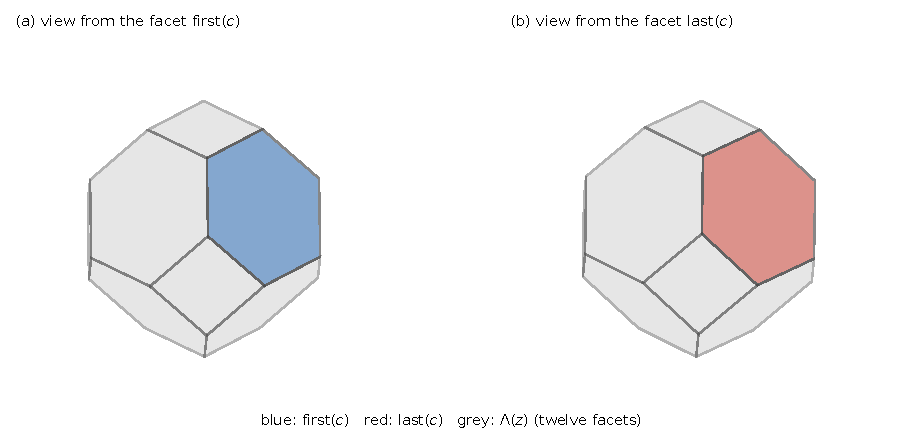
\includegraphics[width=\textwidth]{figures/fig_lift_diagonal.pdf}
\caption{The simplest lift, drawn from exact coordinates. Take the hexagon of $P_3$: its boundary $z$ is a $1$-cycle with the unique filling $c$, so the only lift is the diagonal one. Then $\Lambda(c)$ is the whole permutohedron $P_4$ (a truncated octahedron), $\first(c)$ and $\last(c)$ are the two hexagonal facets at which the new label $3$ is first or last (blue and red), and $\Lambda(z)$ is the band of the remaining twelve facets (grey). The identity $\partial\Lambda(c)=\Lambda(z)+\first(c)+\last(c)$ says that the three pieces together are the boundary sphere of $P_4$ (\cref{lem:LT0}). A non-diagonal lift needs two \emph{different} fillings of $z$.}\label{fig:lift}
\end{figure}

\section{The cochain lift}
\begin{theorem}[cochain lift; computer-assisted obstruction set]\label[theorem]{thm:cochain-lift}
Let $\varphi_2$ be a $2$-cochain of $P_k$ all of whose support faces have the same block $B^\ast$, and put $\varphi_3=\sum_{f\in\operatorname{supp}\varphi_2}\operatorname{Ins}_{B^\ast}(f)$ (add $n$ to the block $B^\ast$). Then for every $2$-cycle $z$ and all fillings $c_1,c_2$,
\[
\varphi_3\bigl(L_{c_1,c_2}(z)\bigr)=\varphi_2(z).
\]
For the anchor pair $(z,\varphi_2)$ of \cref{def:anchor}, $B^\ast=\{2,4,5\}$ and the cochain $\varphi_3$ of weight $6$ has exactly six $4$-faces of $P_7$ with odd boundary pairing, namely $(\{a,2,4,5,6\}\,|\,y\,|\,w)$ with $a\in\{0,1,3\}$ and $(y,w)$ the two orderings of $\{0,1,3\}\setminus\{a\}$ (the six obstructed octahedra of \cref{lem:PS0} with $n=6$ inserted in the first block). Inserting $n$ into \emph{every} block does not work: that cochain pairs to $0$ with $\Lambda(z)$ and has $12$ obstructed $4$-faces.

\end{theorem}
\begin{proof}
The faces of $\first(\cdot)$ and $\last(\cdot)$ have $n$ as a singleton block, whereas every face of $\operatorname{supp}\varphi_3$ has $n$ in the block $B^\ast\cup\{n\}$ of size $\ge2$, so $\varphi_3$ vanishes on $\first(c_1)$ and $\last(c_2)$. The faces $\operatorname{Ins}_i(f)$, $f\in z$, $1\le i\le s$, are pairwise distinct ($\operatorname{Ins}_i(f)$ determines $f$ by deleting $n$ and $i$ as the position of the block carrying $n$), so $\Lambda(z)$ has no cancellation, and $\operatorname{Ins}_i(f)\in\operatorname{supp}\varphi_3$ iff $f\in\operatorname{supp}\varphi_2$ and $B_i=B^\ast$. Hence $\varphi_3(\Lambda(z))=|\operatorname{supp}\varphi_2\cap\operatorname{supp}z|\equiv\varphi_2(z)\pmod2$.
\end{proof}
\begin{corollary}[sufficient condition for a lifted hole]\label[corollary]{cor:lifted-hole}
Let $A$ be a prefix-defined system on seven ranks such that $L=L_{c_1,c_2}(z_{\mathrm{anchor}})$ lies in $K(A)$ and none of the six obstructed $4$-faces of \cref{thm:cochain-lift} lies in $K(A)$. Then $[L]\ne0\in H_3(K(A);\F)$.
\end{corollary}
\begin{proof}
$\varphi_3(\partial G)=0$ for every $4$-face $G$ of $K(A)$ other than the six, so $\varphi_3$ vanishes on $\partial C_4(K(A))$, while $\varphi_3(L)=\varphi_2(z)=1$. Apply the argument of \cref{lem:certificate} one dimension up.
\end{proof}

\section{Certified examples and the arithmetic census}
\begin{proposition}[the $H_3$ examples are lifts; finite-exact]\label[proposition]{prop:H3-examples}
With $B_0=\{21\}$ and $B_1=\{34,38,46\}$ the two small minimal families of the anchor cycle (rank-set numbering as in \cref{app:certs}) and fillings $c_a$ through them, the four $\beta_3=1$ certificates of the seven-label scan at $k=7$ (contents with $x=14$ and $x=15$) are generated by the lift with ordered pairs $(B_0,B_1)$ ($x=15$) and $(B_1,B_0)$ ($x=14$). In each case $P_{z_3}$ coincides with the certificate's $91$ prefix sets and the four minimal filling families coincide (of sizes $1,3,31,33$); in the regime complex the certified $3$-cycle and the lift differ by a boundary.

\end{proposition}
\begin{proposition}[all sixteen lifts of the anchor cycle; finite-exact]\label[proposition]{prop:lift-pairs}
Among the $16$ ordered pairs $(a,b)$ of the four anchor fillings, the four diagonal pairs are degenerate (\cref{thm:lift-cycle}(b), minimal family empty). The twelve off-diagonal pairs have the minimal filling families in $P_7$ whose sizes are listed in \cref{tab:lift-pairs} (4-cell boundaries, at most $38$ free prefix sets of $127$), computed with an independently checked completeness certificate. Reversal $(a,b)\to(b,a)$ preserves the multiset of sizes but not the set $P_{z_3}$.
\begin{table}[ht]\centering\small
\begin{tabular}{@{}lll@{}}\toprule
pair $\{a,b\}$ & sizes of the minimal families & number\\ \midrule
$\{0,1\}$ & $1,3,31,33$ & $4$\\
$\{0,2\}$ & $1,7,15,21$ & $4$\\
$\{0,3\}$ & $2,2,4,16,18,18$ & $6$\\
$\{1,2\}$ & $2,4,4,16,16,18$ & $6$\\
$\{1,3\}$ & $1,3,15,17$ & $4$\\
$\{2,3\}$ & $1,3,3,5$ & $4$\\ \bottomrule
\end{tabular}
\caption{Sizes of the minimal filling families of the twelve off-diagonal lifts (identical for $(a,b)$ and $(b,a)$). Families are in the numbering of the certificates.}\label[proposition]{tab:lift-pairs}
\end{table}

\end{proposition}
\begin{observation}[non-degeneracy across mechanisms; finite-exact]\label[observation]{obs:nondeg}
For each of the $32$ law classes of \cref{obs:atlas} and each of the $554$ ordered off-diagonal pairs of minimal fillings $(a\ne b)$, the lift is non-degenerate: it does not bound in the complex generated by its own prefix sets. All $146$ diagonal lifts are degenerate, as \cref{thm:lift-cycle}(b) requires. A general proof is not known: it would show that the \emph{bridge chains} $\Lambda(c_a)$, $\Lambda(c_b)$ are not contained in $K(P_L)$ (so that the reduction $L\simeq\last(c_a+c_b)$ of \cref{thm:lift-cycle}(c) is unavailable), which was confirmed for the twelve anchor pairs.

\end{observation}
\begin{observation}[arithmetic survival of the lifts; bounded]\label[observation]{obs:AS1}
Identity role map, all $1{,}560{,}780$ seven-label contents with labels in $[2,30]$, twelve patterns: $202$ contents admit a hole regime for at least one lifted pattern (by pattern: $01$: $70$; $02$: $39$; $03$: $13$; $10$: $77$; $12$: $22$; $20$: $46$; $21$: $25$; $30$: $18$; none for $13,23,31,32$), against the $4$ contents found at labels $\le18$ by the first scan. All $214$ predicted regimes were verified on the full regime complexes: $z_3$ present, not a boundary, $\beta_3\in\{1\ (198),\,2\ (6),\,3\ (9),\,4\ (1)\}$, each with an exact cochain; $100$ random predicted negatives bounded. Two hundred of the $202$ contents have a six-label sub-content with an $H_2$ hole (the two exceptions have $x=30$). Odd $x$ mostly select patterns $(a,b)$ with $a<b$, even $x$ the reverse ($167$ of $202$); this is not a theorem.

\end{observation}
Only the anchor class was censused for lifts. Whether every $H_3$ regime of a seven-label content is a lift is not known; the census covers only lifted patterns.

\section{Filling dependence}\label{sec:filldep}
The lift depends on two fillings. Is its homology class an invariant of $z$ alone, or does it remember how $z$ was filled? The answer is exact.
\begin{theorem}[filling dependence]\label[theorem]{thm:filling-dependence}
Let $z$ be a $2$-cycle of $P_6$ and $c_a,c_a',c_b,c_b'$ fillings of $z$. Write $L_{a,b}=L_{c_a,c_b}(z)$ and, for a $3$-cycle $d$ of $P_6$, regard $\first(d),\last(d)$ as $3$-cycles of $P_7$.
\begin{enumerate}[label=\textup{(FI-\arabic*)}]
\item $L_{a',b}+L_{a,b}=\first(c_a+c_a')$ and $L_{a,b'}+L_{a,b}=\last(c_b+c_b')$.
\item Let $A$ be a prefix-defined system with $K(A)\supseteq\operatorname{supp}L_{a,b}\cup\operatorname{supp}L_{a',b}$. Then $[L_{a',b}]=[L_{a,b}]\in H_3(K(A))$ iff $\first(d)\in\partial C_4(K(A))$, $d=c_a+c_a'$. This is the sharp criterion, not a sufficient condition.
\item For a $3$-cycle $d$: $\partial\Lambda(d)=\first(d)+\last(d)$; hence $[\first(d)]=[\last(d)]$ in every $K(A)$ containing the cells of $\Lambda(d)$.
\item $L_{a,a'}=L_{a',a'}+\first(c_a+c_{a'})$ and $L_{a',a'}=\partial\Lambda(c_{a'})$; so $[L_{a,a'}]=[\first(d)]$ in every $K(A)$ containing the cells of $\Lambda(c_{a'})$.
\end{enumerate}

\end{theorem}
\begin{proof}
(FI-1): $\first$ and $\last$ are additive; $L_{a',b}+L_{a,b}=\first(c_a')+\first(c_a)$. (FI-2): two cycles of $K(A)$ are homologous in $K(A)$ iff their sum is in $\partial C_4(K(A))$; their sum is $\first(d)$ by (FI-1), whose cells are among the cells of the two lifts. (FI-3): \cref{lem:LT0} gives $\partial\Lambda(d)=\Lambda(\partial d)+\first(d)+\last(d)$ and $\partial d=0$. (FI-4): (FI-1) with $b=a'$ gives the first identity, \cref{thm:lift-cycle}(b) the second.
\end{proof}
\begin{theorem}[certified filling dependence for the anchor; finite-exact]\label[theorem]{thm:FI-anchor}
For the anchor cycle with its four minimal fillings $c_0,\dots,c_3$ (through $B_0,\dots,B_3$):
\begin{enumerate}[label=(\roman*)]
\item \emph{Within a family.} Every filling in $K(P_z\cup B_i)$ differs from $c_i$ by a $3$-cycle $d$ of that complex ($\dim Z_3=9,9,25,31$); $\first(d)$ bounds in its own complex for all $511+511$ nonzero $d$ ($B_0,B_1$, exhaustive) and for the $31+25$ basis elements plus $2000$ random sums each ($B_2,B_3$). So the lift class does not depend on the filling chosen within a family.
\item \emph{Between families.} For $\{i,j\}\in\{01,02,13,23\}$ the cycle $\first(c_i+c_j)$ has the empty family (it is self-bounding), so $[L_{i,b}]=[L_{j,b}]$ in every complex containing both. For $\{0,3\}$ and $\{1,2\}$ it has exactly two single-prefix-set minimal families ($\{89\},\{102\}$ resp.\ $\{85\},\{106\}$) plus two of size $62$; independence holds iff $A$ contains one of them.
\item \emph{Realised dependence.} In $K(P_L\cup P_{L'})$ the classes $[L],[L'],[L+L']$ are all nonzero for $\{a,a'\}=\{0,3\}$ ($b=1,2$) and $\{1,2\}$ ($b=0,3$). Arithmetic realisations (identity role map): content $(2,3,8,9,14,15,20)$ at $m=33600$ and $(3,8,9,14,15,20,21)$ at $m=793800$, pair $(a,a';b)=(1,2;0)$ and $(2,1;0)$: $L_{1,0}$, $L_{2,0}$ and their sum are non-bounding against all admitted $4$-faces, i.e. two linearly independent $H_3$ classes from two minimal fillings of one $H_2$ cycle.
\end{enumerate}
No universal independence theorem is true; (FI-2) is the exact criterion. Independence criteria for the other $31$ classes, integral coefficients, and whether dependence occurs for $\{0,3\}$/$\{1,2\}$ arithmetically beyond the two witnesses (none other found among the $202$ seeds) are open.

\end{theorem}
\emph{Does the topology of a generative history space depend only on which lower-dimensional cycles can be filled, or also on the relations between their alternative fillings?} By \cref{thm:filling-dependence,thm:FI-anchor} it depends also on the relations, and exactly through whether $\first(c_a+c_a')$ bounds in the complex.

\section{Iterated lifts and role maps}
\begin{theorem}[iterated lift]\label[theorem]{thm:iterated-lift}\leavevmode
\begin{enumerate}[label=(HL-\arabic*)]
\item \emph{(proved)} For a $3$-cycle $w$ of $P_7$ and $4$-chains $c,c'$ with $\partial c=\partial c'=w$, $L^2=\Lambda(w)+\first(c)+\last(c')$ is a $4$-cycle of $P_8$, and the diagonal $L^2_{c,c}=\partial\Lambda(c)$ bounds.
\item \emph{(finite-exact)} For the base $w=L_{0,1}$ the fillings index pairs $(0,1),(1,0),(0,2)$ give non-degenerate $4$-cycles (weights $2146,2146,2418$; $187,187,215$ prefix sets), whereas $(0,0)$ bounds in its own complex.
\item \emph{(bounded; one certified example)} Content $(2,3,4,5,8,9,15,20)$ at $m=86400$, pair $(0,1)$, fillings $(1,0)$: an explicit $2146$-face $4$-cycle together with a $6$-face cochain $\varphi$ with $\varphi(L^2)=1$ and $\varphi\circ\partial=0$ on all $3819$ admitted $5$-faces, checked by an elimination-free verifier. Seven further contents are verified identically. All come from the first seed content $(2,3,4,5,8,9,15)$ of the seed list; the scan stopped after $5$ hits and is not a census.
\end{enumerate}

\end{theorem}
\begin{proof}[Proof of (HL-1)]
\Cref{lem:LT0} and \cref{thm:lift-cycle}(a)--(b) use only that $n$ is a new rank on any permutohedron $P_k$, $k\ge2$; apply them with $P_7$ in place of $P_6$ and $n=7$.
\end{proof}
\begin{observation}[role-map correction; finite-exact]\label[observation]{obs:rolemap}
The seven-label census used the identity role map: the six-label sub-content carries the anchor cycle on ranks $0,\dots,5$ as given. For both sub-contents $(2,9,15,20,26,27)$ and $(8,9,15,20,26,27)$ the identity image has no $H_2$ regime, but $18$ of the $180$ $S_6$-images of the anchor class do. The statement that the lift does not require the lower-dimensional hole to survive is therefore supported for the identity role map only; the role-invariant version is not established.

\end{observation}

\section{The filling-dependence map}\label{sec:JX}
\begin{definition}\label[definition]{def:JX}
Let $X=K_{k+1}(A)$ and $j\ge1$. Put $V_X=\{d\in Z_j(P_k):\ \first(d)\in C_j(X)\}$, $J_X:V_X\to H_j(X)$, $d\mapsto[\first(d)]$, and $r_{\mathrm{fill}}(X)=\dim\operatorname{im}J_X$. By (FI-1) the lifts with first filling $c_a+d$, $d\in V_X$, have classes $[L]+J_X(d)$, so $r_{\mathrm{fill}}$ counts the independent directions of filling dependence.
\end{definition}
\begin{theorem}[facet theorem and retraction criterion]\label[theorem]{thm:JX}
Let $n$ be the new rank, $A'=\{I:\ I\cup\{n\}\in A\}$ and $F_X=\{f:\ \first(f)\in X\}$.
\begin{enumerate}[label=(J-\arabic*)]
\item \emph{(facet theorem, proved)} $\first,\last$ are injective, dimension-preserving chain maps $P_k\to P_{k+1}$, $\Pref(\first(f))=\{\{n\}\}\cup\{I\cup\{n\}:I\in\Pref(f)\}$, and $F_X=K_k(A')$ (empty unless $\{n\}\in A$). Hence $V_X=Z_j(F_X)$, $J_X$ factors through $H_j(F_X)$ and equals $\first_\ast:H_j(F_X)\to H_j(X)$, so $r_{\mathrm{fill}}(X)\le\beta_j(F_X)$. The same holds for $\last$ with $A''$.
\item \emph{(retraction criterion, proved)} Define $\rho(g)=g\setminus\{n\}$ if $\{n\}$ is a singleton block of $g$ and $\rho(g)=0$ otherwise. Over $\F$, $\rho$ is a dimension-preserving chain map $P_{k+1}\to P_k$ with $\rho\circ\first=\mathrm{id}$. Consequently $\ker J_X\subseteq Z_j(F_X)\cap\partial C_{j+1}(G_X)$, $G_X=\rho(X_{\mathrm{sing}})$ ($X_{\mathrm{sing}}$ the faces of $X$ with $\{n\}$ a block), giving
\[
\dim Z_j(F_X)-\dim\bigl(Z_j(F_X)\cap\partial C_{j+1}(G_X)\bigr)\ \le\ r_{\mathrm{fill}}(X)\ \le\ \beta_j(F_X).
\]
If $\rho(X)\subseteq F_X$ (condition RET) then $\first_\ast$ is split injective and $r_{\mathrm{fill}}=\beta_j(F_X)$.
\item \emph{(finite-exact)} Over the $310$ surviving lift instances ($202$ seed contents $\times$ twelve off-diagonal anchor patterns, at $m=K_P$): $r_{\mathrm{fill}}\in\{0,1\}$ and $r_{\mathrm{fill}}=\beta_3(F_X)$ in all $310$ ($298$ with $0$, $12$ with $1$); the lower bound of (J-2) equals $r_{\mathrm{fill}}$ in all $310$ (the sandwich is tight), while RET fails in all $310$. So injectivity of $\first_\ast$ is proved instance by instance and not by a global retraction. $\dim V_X=37$ in all $12$ instances with $r_{\mathrm{fill}}=1$.
\item \emph{(finite-exact; witnesses)} For $(2,3,8,9,14,15,20)$ at $m=33600$ and $(3,8,9,14,15,20,21)$ at $m=793800$: $\dim V_X=37$, $r_{\mathrm{fill}}=1$, $\dim\ker J_X=36$; exactly $2^1$ lifted classes are attainable by varying the first filling. In the scan $m=Kt$, $t=1,\dots,60$, $r_{\mathrm{fill}}\in\{0,1\}$: the dependence appears and disappears with the complex.
\item \emph{(finite-exact; second lift)} At $H_4$ ($P_7\to P_8$) for the eight certified contents: $r_{\mathrm{fill}}=0$ for both $\first$ and $\last$ ($\dim V_X\in\{54,57,72\}$ resp.\ $\{54,57,79,98\}$ and $\beta_4(F_X)=0$). The dependence found in degree $3$ did \emph{not} propagate to degree $4$ in these complexes; this is a scoped observation, not a theorem that it cannot.
\item \emph{(proved, conditional wording)} For a fixed base lift and second filling, with all fillings in $V_X$ admitted, the number of attainable lifted classes is $2^{r_{\mathrm{fill}}(X)}$ (an affine coset of $\operatorname{im}J_X$, by (FI-1)). A Shannon-entropy reading ($r_{\mathrm{fill}}$ bits) needs an explicit uniform-measure convention; in all $310$ instances there is at most $1$ bit.
\item \emph{(open)} Why $\first_\ast$ is injective in all $310$ instances; a structural description of $A'=\{I:D(I\cup\{n\})\mid m\}$ and of $\beta_3(K_6(A'))$ in terms of gates; the relation $\first_\ast\approx\last_\ast$ via $\Lambda$; integral and torsion coefficients; a propagation theorem $j\to j+1$.
\end{enumerate}

\end{theorem}
\begin{proof}[Proof of (J-1), (J-2), (J-6)]
\emph{(J-1).} The block $\{n\}$ of $\first(f)$ is a singleton and cannot be split, so $\partial\first(f)=\first(\partial f)$, likewise for $\last$; injectivity and the formula for $\Pref$ are read off the definition of prefixes of $(\{n\}|f)$. $\first(f)\in X$ iff $\Pref(\first f)\subseteq A$ iff $\{n\}\in A$ and $I\cup\{n\}\in A$ for all $I\in\Pref(f)$ iff $\{n\}\in A$ and $f\in K_k(A')$. A class $d\in B_j(F_X)$, $d=\partial e$ with $e\in C_{j+1}(F_X)$, gives $\first(d)=\partial\first(e)$ with $\first(e)\in C(X)$, so $J_X$ vanishes on $B_j(F_X)$ and $r_{\mathrm{fill}}=\dim Z_j(F_X)-\dim\ker J_X\le\dim Z_j-\dim B_j=\beta_j(F_X)$.
\emph{(J-2).} If $n$ is a singleton block of $g$, splits of other blocks keep $n$ a singleton and commute with deleting $n$, and the block $\{n\}$ cannot split; hence $\partial\rho(g)=\rho(\partial g)$. If $n$ lies in a block $B=U\cup\{n\}$ with $|B|\ge2$, then $\rho(g)=0$; in $\partial g$, splits of other blocks and splits of $B$ keeping $n$ in a block of size $\ge2$ are killed by $\rho$, and the only surviving terms are the splits $(\{n\}|U)$ and $(U|\{n\}),$ which both delete to the same face and cancel mod $2$, so $\rho(\partial g)=0$. Thus $\rho$ is a chain map, and $\rho\circ\first=\mathrm{id}$. If $\first(d)=\partial w$ with $w\in C(X)$, then $d=\rho(\first d)=\rho(\partial w)=\partial\rho(w)$ with $\rho(w)\in C(G_X)$, so $\ker J_X\subseteq Z_j(F_X)\cap\partial C_{j+1}(G_X)$, which gives the lower bound. Under RET, $\rho(w)\in C(F_X)$, so $d\in B_j(F_X)$ and $\ker J_X=B_j(F_X)$.
\emph{(J-6).} If $\first(c_a)\in C(X)$ then $\first(c_a+d)\in C(X)$ iff $\first(d)\in C(X)$ iff $d\in V_X$; by (FI-1) the class of the lift with first filling $c_a+d$ is $[L]+J_X(d)$.
\end{proof}
The lifted homology therefore depends on two things: \emph{which} cycles fill (the survival laws of \cref{thm:AT1}), and the lower-dimensional homology of the first-facet complex $F_X$, the freedom of filling relations being exactly the part of $H_j(F_X)$ that survives in $H_j(X)$.

\section{Scope of the lift results}
General-dimension statements are limited to the chain-level calculus: \cref{lem:LT0}, \cref{thm:lift-cycle}, \cref{thm:filling-dependence}, parts (J-1), (J-2) and (J-6) of \cref{thm:JX}, and part (HL-1) of \cref{thm:iterated-lift}. Everything that names a content is finite or bounded: non-degeneracy of the off-diagonal lifts is verified for $554$ pairs but not proved in general, injectivity of $\first_\ast$ is verified instance by instance, and the four-dimensional example is a certified single content with seven further verified neighbours. Figure~\ref{fig:lift} and the tables above are evidence about the anchor class and the identity role map at labels $\le30$, not a classification of $H_3$.
